% w nawiasie kwadratowym wpisujemy rodzaj pracy: 
% magisterska, licencjacka, inzynierska
\documentclass[magisterska]{pracadypl}

%% ważne definicje %%
\usepackage{tgtermes}
\usepackage[T1]{fontenc}
\usepackage{polski}
\usepackage[utf8]{inputenc}
\input glyphtounicode
\pdfgentounicode=1
\usepackage{amssymb}
\usepackage{amsmath}
\usepackage{caption}
\usepackage{graphicx}
\setcounter{secnumdepth}{4}  % Ensure subsubsection is numbered
\setcounter{tocdepth}{4}     % Ensure subsubsection appears in TOC
\usepackage{titlesec}
\usepackage{color}
\usepackage{xcolor}
\usepackage{float}
\usepackage{listings}
\usepackage{parskip}
\usepackage{xcolor} % optional, for color
\usepackage{chngcntr}
\counterwithout{figure}{chapter}
\bibliographystyle{plain}

\def\mgr{magisterska}
\def\lic{licencjacka}
\def\inz{inżynierska}

\def\sk{Słowa kluczowe}
\def\kw{Keywords}
\def\et{Title in English}
%% koniec ważnych definicji %%

%% wypełnia Autor pracy %%

%autor pracy
\author{Gabriel Ozeg}
%numer albumu
\nralbumu{395263}
%tytuł pracy
\title{System antykolizyjny na mikroprocesorze Raspberry Pi}
%kierunek studiów
\kierunek{Informatyka}
%promotor w dopełniaczu
\opiekun{dr Paweł Zajączkowski}
\katedra{Katedra Informatyki Stosowanej}
%rok
\date{2025}
%Słowa kluczowe:
\slkluczowe{Przetwarzanie obrazu, Głębia obrazu, Metody pomiaru odległości w czasie rzeczywistym, Zastosowania w robotyce}
%tytuł po angielsku
\tytulang{Collision avoidance system on Raspberry Pi microprocessor}
%słowa kluczowe po angielsku
\keywords{Image Processing, Image Depth, Real-Time Distance Measurement Methods, Applications in Robotics}
%% koniec ważnych definicji %%

%% APD %%
%% w systemie APD należy jeszcze wpisać, poza powyższymi informacjami, streszczenie oraz streszczenie w języku angielskim  %%


%%% definicje %%%
\def\pd{\noindent \textbf{Dowód.~}} %%początek dowodu
\def\kd{\hfill\mbox{$\rule{2mm}{2mm}$}} %%koniec dowodu
\newtheorem{defi}{Definicja}[section]
\newtheorem{uwaga}{Uwaga}[section]
\newtheorem{tw}{Twierdzenie}[section]
\newtheorem{lem}{Lemat}[section]
\newtheorem{wn}{Wniosek}[section]
\renewcommand\thetw{\thesection.\arabic{tw}.}
\renewcommand\thedefi{\thesection.\arabic{defi}.}
\renewcommand\theuwaga{\thesection.\arabic{uwaga}.}
\renewcommand\thetw{\thesection.\arabic{tw}.}
\renewcommand\thelem{\thesection.\arabic{lem}.}
\renewcommand\thewn{\thesection.\arabic{wn}.}
%
\definecolor{wmiigreen}{rgb}{0.0, 0.5, 0.0}
\titleformat{\chapter}[display]
  {\normalfont\huge\bfseries\color{wmiigreen}}{\chaptertitlename\ \thechapter}{10pt}{\Huge}
 %
\linespread{1.3}
%%% koniec definicji %%%


\lstdefinestyle{mypython}{
    language=Python,
    basicstyle=\ttfamily\scriptsize,
    keywordstyle=\color{red}\bfseries,
    stringstyle=\color{green},
    commentstyle=\color{blue},
}

\begin{document}

\maketitle
\tableofcontents
\newpage

\chapter{Wstęp}

Przetwarzanie obrazu to dziedzina informatyki i inżynierii zajmująca się analizą, modyfikacją i interpretacją obrazów cyfrowych za pomocą metod numerycznych i algorytmów komputerowych. Jej celem jest poprawa jakości obrazów, ekstrakcja informacji, segmentacja obiektów lub ich klasyfikacja. Przetwarzanie obrazu znajduje zastosowanie w wielu obszarach, takich jak medycyna (np. analiza zdjęć RTG), przemysł (np. kontrola jakości), bezpieczeństwo (np. rozpoznawanie twarzy), robotyka oraz systemy wizyjne pojazdów autonomicznych. Dzięki połączeniu technik matematycznych, statystycznych i sztucznej inteligencji możliwe jest coraz bardziej precyzyjne i automatyczne rozumienie zawartości obrazów.

\chapter{Część główna}

\section{+Natura kamery}

Kamery rejestrują promienie świetlne z otoczenia. Zasadniczo kamera działa podobnie jak ludzkie oko — odbite promienie światła trafiają do oka i są skupiane na siatkówce.

Najprostszym modelem kamery jest tzw. „kamera otworkowa”. To dobre uproszczenie pozwalające zrozumieć podstawy działania kamery. W tym modelu wszystkie promienie świetlne są blokowane przez ścianki, a tylko te przechodzące przez mały otwór trafiają na powierzchnię światłoczułą wewnątrz kamery, tworząc odwrócony obraz. Poniższa ilustracja przedstawia tę zasadę.

\begin{figure}[H]
    \centering
    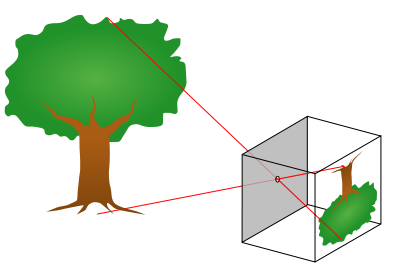
\includegraphics[width=0.5\textwidth]{images/light.png}
    \captionsetup{font=footnotesize}
    \caption[Odwrócenie obrazu przez soczewkę. https://funsizephysics.com/use-light-turn-world-upside/]{Odwrócenie obrazu przez soczewkę}
    \label{fig:rpi}
\end{figure}

Choć ten model jest prosty, nie nadaje się dobrze do rejestrowania wystarczającej ilości światła przy krótkim czasie naświetlania. Dlatego w kamerach stosuje się soczewki, które skupiają promienie świetlne w jednym punkcie. Niestety, powoduje to powstawanie zniekształceń.

Istnieją dwa główne rodzaje zniekształceń:

\begin{itemize}
  \item Zniekształcenie promieniowe(radialne) — spowodowane kształtem soczewki,występujące symetrycznie względem środka obrazu.

  \item Zniekształcenie styczne(tangencjalne) — wynikające z niedoskonałości montażu lub geometrii kamery.
\end{itemize}

Obrazy zniekształcone w ten sposób można skorygować za pomocą metod matematycznych. Proces kalibracji pozwala stworzyć model geometrii kamery oraz model zniekształceń obiektywu. Te modele określają tzw. parametry wewnętrzne kamery.

\subsection{+Ogniskowa obiektywu}

Względny rozmiar obrazu rzutowanego na powierzchnię w kamerze zależy od ogniskowej.

W modelu otworkowym ogniskowa to odległość między otworem, przez który przechodzi światło, a obszarem, na który rzutowany jest obraz.

Aby wyznaczyć, jak duży będzie obraz obiektu na płaszczyźnie projekcji, korzystamy z \textbf{twierdzenia Talesa}.  
Dlaczego?

Obiekt znajdujący się w przestrzeni oraz jego rzut w kamerze tworzą dwa \textbf{podobne trójkąty}:
\begin{itemize}
    \item Jeden utworzony przez obiekt o wysokości \( X \), znajdujący się w odległości \( Z \) od kamery.
    \item Drugi utworzony przez obraz tego obiektu na płaszczyźnie znajdującej się w odległości \( f \) od otworu kamery, którego wysokość to \( x \).
\end{itemize}

Ponieważ kąty tych trójkątów są identyczne (wierzchołek kąta w otworze kamery) i odpowiadające sobie boki są proporcjonalne, możemy zastosować twierdzenie Talesa:

\[
\frac{x}{f} = \frac{X}{Z} \Rightarrow x = f \cdot \frac{X}{Z}
\]

Obraz na matrycy jest odwrócony, dlatego często w literaturze pojawia się wersja ze znakiem minus:

\[
-x = f \cdot \frac{X}{Z}
\]

\begin{itemize}
  \item \textbf{$x$}: obraz obiektu (znak minus wynika z tego, że obraz jest odwrócony)
  \item \textbf{$X$}: rozmiar obiektu
  \item \textbf{$Z$}: odległość od otworu do obiektu
  \item \textbf{$f$}: ogniskowa, odległość od otworu do obrazu
\end{itemize}

\begin{figure}[H]  % 'h' means "here", it places the figure at the current location in the document
    \centering  % Centers the image
    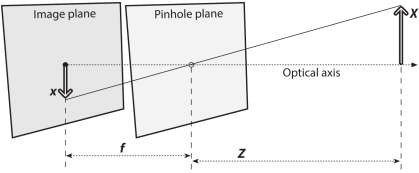
\includegraphics[width=0.5\textwidth]{images/pinhole.png}  % Adjust the path and width as necessary
    \captionsetup{font=footnotesize}
    \caption[Model kamery otworkowej. Learning OpenCV 3, O'Reilly, Str. 639]{Model kamery otworkowej}
    \label{fig:rpi}  % Optional: use to refer to this image later in the text
\end{figure}

Ponieważ soczewka nie jest idealnie wyśrodkowana, wprowadzono dwa parametry, $C_x$ i $C_y$, oznaczające odpowiednio poziome i pionowe przemieszczenie soczewki.
Ogniskowa na osiach $X$ i $Y$ są również różna, ponieważ obszar obrazu jest prostokątny. Daje to następujący wzór na położenie obiektu na powierzchni.

\[
x_{\text{screen}} = f_x \left( \frac{X}{Z} \right) + c_x, \quad
y_{\text{screen}} = f_y \left( \frac{Y}{Z} \right) + c_y
\]

Rzutowane punkty świata rzeczywistego na powierzchnię obrazu można zatem modelować w następujący sposób. $M$ jest tutaj macierzą wewnętrzną.

\bigskip

Punkt w przestrzeni 3D:
\[
Q = \begin{bmatrix} X \\ Y \\ Z \end{bmatrix}
\]

Po rzutowaniu za pomocą macierzy kamery $M$:
\[
M = \begin{bmatrix}
f_x & 0 & c_x \\
0 & f_y & c_y \\
0 & 0 & 1
\end{bmatrix}
\]

otrzymujemy punkt obrazu w jednorodnych współrzędnych:
\[
q = M \cdot \begin{bmatrix}
\frac{X}{Z} \\
\frac{Y}{Z} \\
1
\end{bmatrix}
=
\begin{bmatrix}
f_x \cdot \frac{X}{Z} + c_x \\
f_y \cdot \frac{Y}{Z} + c_y \\
1
\end{bmatrix}
\]

Po normalizacji współrzędnych jednorodnych:
\[
x = \frac{q_x}{q_w} = f_x \cdot \frac{X}{Z} + c_x
\quad , \quad
y = \frac{q_y}{q_w} = f_y \cdot \frac{Y}{Z} + c_y
\]

Dla ogólnej macierzy projekcji:
\[
P = M \cdot [R \;|\; t]
\]

Macierz \( P = M[R | t] \) nazywana jest macierzą projekcji kamery i zawiera zarówno informacje o parametrach wewnętrznych kamery (macierz \( M \)), jak i jej położeniu i orientacji w przestrzeni (macierze \( R \) i \( t \)).

Rzut punktu \( Q_h = \begin{bmatrix} X \\ Y \\ Z \\ 1 \end{bmatrix} \) przy pomocy tej macierzy daje nam współrzędne punktu\\ \( q = \begin{bmatrix} x' \\ y' \\ w \end{bmatrix} \) w jednorodnych współrzędnych, które po znormalizowaniu (\( x = \frac{x'}{w} \)) dają końcowe położenie punktu na obrazie.

\[
x = \frac{x'}{w}, \quad y = \frac{y'}{w}
\]

Współrzędne \( x, y \) po normalizacji są współrzędnymi piksela na płaszczyźnie obrazu, czyli miejscem, gdzie dany punkt 3D zostanie odwzorowany na zdjęciu lub klatce z kamery. Uwzględniają one zarówno parametry geometryczne obiektywu (ogniskowe \( f_x, f_y \)) jak i przesunięcia optycznego środka obrazu (\( c_x, c_y \)).

\subsection{Dystorsja obrazu}

\begin{figure}[H]  % 'h' means "here", it places the figure at the current location in the document
    \centering  % Centers the image
    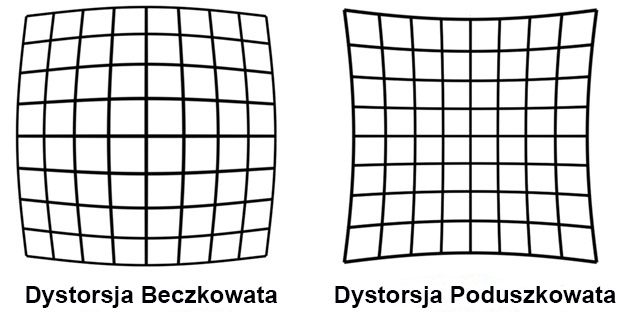
\includegraphics[width=0.5\textwidth]{images/dystorsje.png}  % Adjust the path and width as necessary
    \captionsetup{font=footnotesize}
    \caption[Rodzaje dystorsji. https://beafoto.pl/dystorsja]{Rodzaje dystorsji}
    \label{fig:rpi}  % Optional: use to refer to this image later in the text
\end{figure}

Teoretycznie możliwe jest zbudowanie obiektywu, który nie powoduje zniekształceń, np. przy użyciu soczewki parabolicznej. W praktyce jednak znacznie łatwiej i taniej jest wytwarzać soczewki sferyczne, które niestety powodują różne typy zniekształceń geometrycznych obrazu.

Aby móc opisać i skorygować te zniekształcenia, punkt obrazu wyrażony w pikselach \( (u, v) \) przekształca się najpierw do znormalizowanego układu współrzędnych kamery:

\[
x = \frac{u - c_x}{f_x}, \quad y = \frac{v - c_y}{f_y}
\]

Gdzie:
\begin{itemize}
    \item \( (c_x, c_y) \) — współrzędne głównego punktu optycznego (środka obrazu),
    \item \( (f_x, f_y) \) — ogniskowe w poziomie i pionie wyrażone w pikselach,
    \item \( (x, y) \) — znormalizowane współrzędne względem osi optycznej kamery.
\end{itemize}

\subsection*{Zniekształcenia promieniowe i rozwinięcie Taylora}

Zniekształcenia promieniowe (ang. \emph{radial distortion}) są symetryczne względem środka obrazu i ich wpływ rośnie wraz z odległością od środka. Dla punktów znormalizowanych odległość ta dana jest przez:

\[
r^2 = x^2 + y^2
\]

Efekt zniekształcenia można modelować jako nieliniową funkcję \( D(r) \), która modyfikuje współrzędne punktu zależnie od \( r \). Ponieważ funkcja \( D(r) \) nie jest znana analitycznie, stosujemy jej rozwinięcie Taylora w punkcie \( r = 0 \):

\[
D(r) = 1 + k_1 r^2 + k_2 r^4 + k_3 r^6 + \ldots
\]

Ograniczamy się zwykle do trzeciego rzędu (\( r^6 \)), ponieważ kolejne składniki mają marginalny wpływ, a zwiększają złożoność obliczeń. Po uwzględnieniu tej funkcji korekta zniekształcenia promieniowego ma postać:

\begin{align*}
x_{\text{radial}} &= x \cdot \left(1 + k_1 r^2 + k_2 r^4 + k_3 r^6 \right) \\
y_{\text{radial}} &= y \cdot \left(1 + k_1 r^2 + k_2 r^4 + k_3 r^6 \right)
\end{align*}

\subsection*{Zniekształcenia styczne (tangencjalne)}

Zniekształcenia styczne pojawiają się w wyniku niewspółosiowości soczewek (np. przesunięcia lub nachylenia względem osi optycznej). Ich model opiera się na dwóch parametrach \( p_1 \) i \( p_2 \):

\begin{align*}
x_{\text{tangential}} &= x + \left[2p_1 x y + p_2 (r^2 + 2x^2)\right] \\
y_{\text{tangential}} &= y + \left[p_1 (r^2 + 2y^2) + 2p_2 x y\right]
\end{align*}

\subsection*{Pełna korekta punktu znormalizowanego}

Sumując oba typy zniekształceń, uzyskujemy skorygowane współrzędne punktu w układzie znormalizowanym:

\begin{align*}
x_{\text{corrected}} &= x(1 + k_1 r^2 + k_2 r^4 + k_3 r^6) + 2p_1 x y + p_2 (r^2 + 2x^2) \\
y_{\text{corrected}} &= y(1 + k_1 r^2 + k_2 r^4 + k_3 r^6) + p_1 (r^2 + 2y^2) + 2p_2 x y
\end{align*}

\subsection*{Powrót do współrzędnych obrazu}

Na końcu przekształcamy punkt z powrotem do układu pikselowego:

\[
u_{\text{corrected}} = f_x \cdot x_{\text{corrected}} + c_x, \quad
v_{\text{corrected}} = f_y \cdot y_{\text{corrected}} + c_y
\]

W ten sposób otrzymujemy ostateczną, skorygowaną pozycję punktu obrazu, która uwzględnia wpływ obu typów zniekształceń optycznych.

\subsection{Dane z obrazu kamery}

Znormalizowane współrzędne $(x, y)$ oraz współrzędne pikselowe $(u, v)$ służą do różnych celów, ale są ze sobą ściśle powiązane. Współrzędne znormalizowane są używane wszędzie tam, gdzie istotna jest struktura geometryczna sceny i relacje przestrzenne – np. w algorytmach rekonstrukcji 3D, lokalizacji kamery czy kalibracji. Z kolei współrzędne pikselowe są wykorzystywane do interakcji z obrazem: lokalizacji punktów na zdjęciu, wizualizacji, wykrywania cech czy ekstrakcji informacji wizualnych.

\section{Rodzaje kamer i technik używane do estymacji głębi}

\subsection{Monocular Vision}

\begin{figure}[H]  % 'h' means "here", it places the figure at the current location in the document
    \centering  % Centers the image
    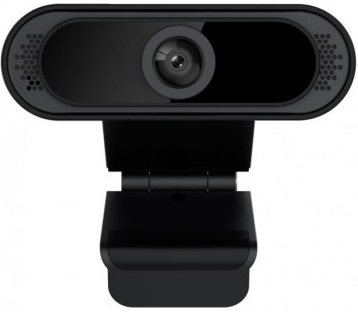
\includegraphics[width=0.2\textwidth]{images/MONO.png}  % Adjust the path and width as necessary
    \captionsetup{font=footnotesize}
    \caption[Kamerka internetowa. https://cell-kom.com/inne/21454-kamera-internetowa-full-hd-b16-1080p-5900217390350.html]{Kamerka internetowa.}
    \label{fig:mono}  % Optional: use to refer to this image later in the text
\end{figure}

Monocular vision (widzenie monokularne) to technika pozyskiwania informacji wizualnych przy użyciu tylko jednej kamery, czyli takiej, która rejestruje obraz z pojedynczego punktu widzenia — podobnie jak jedno oko u człowieka.
W przypadku obrazu monokularnego, każdy piksel dostarcza jedynie informacji o jasności i kolorze w płaszczyźnie 2D. Brakuje natomiast bezpośredniej informacji o głębokości, czyli odległości od kamery. Z tego względu estymacja głębi z pojedynczego obrazu jest niedookreślonym problemem inwersyjnym – wiele różnych trójwymiarowych scen może prowadzić do identycznej projekcji 2D.

Aby rozwiązać ten problem, konieczne jest wprowadzenie priorytetów – dodatkowych założeń na temat struktury świata, geometrii sceny lub charakterystyki obiektów. Przykładowe priorytety to:

\begin{itemize}
  \item Zakładanie horyzontalności podłoża i pionowości ścian.

  \item Regularność obiektów (np. ludzie mają podobną wysokość).

  \item Perspektywa (linie zbiegające się w punkcie zbiegu sugerują głębię).

  \item Znajomość statystycznych regularności obrazów.
\end{itemize}

Z matematycznego punktu widzenia, obraz monokularny powstaje na skutek rzutowania sceny trójwymiarowej na płaszczyznę dwuwymiarową za pomocą rzutowania perspektywicznego. Każdy punkt $P = (X,Y,Z)$ w przestrzeni 3D odwzorowany jest na punkt $p = (x,y)$ w obrazie 2D zgodnie z wzorami:

\[
x = f \cdot \frac{X}{Z}, \quad
y = f \cdot \frac{Y}{Z}
\]

gdzie $f$ to ogniskowa kamery, a $Z$ to głębokość. Zauważmy, że głębokość $Z$ znajduje się w mianowniku, co oznacza, że jej zmiany mają kluczowy wpływ na rozmiar i położenie obiektów na obrazie.

W kontekście wizji monokularnej, głębokie uczenie odgrywa kluczową rolę, umożliwiając estymację głębi, rekonstrukcję scen 3D czy detekcję obiektów na podstawie pojedynczego obrazu. Zamiast polegać na klasycznych metodach geometrycznych, takich jak triangulacja czy analiza ruchu, sieci neuronowe uczą się z dużych zbiorów danych, wychwytując złożone wzorce i zależności przestrzenne. Mimo wysokiej skuteczności, tego typu podejścia mają swoje ograniczenia – wymagają dużej mocy obliczeniowej, są podatne na błędy przy nietypowych danych wejściowych, a ich efektywność jest ściśle związana z jakością i zakresem danych użytych do treningu.

\begin{minipage}[t]{\textwidth}
\textbf{Wady i ograniczenia:}
\begin{itemize}
  \item Brak absolutnej skali – z jednego obrazu nie można jednoznacznie wywnioskować rzeczywistej odległości.

  \item Trudności w teksturowo jednorodnych obszarach – gdzie brak cech uniemożliwia dobre przewidywanie.

  \item Problemy z generalizacją – modele trenowane na jednej dziedzinie mogą słabo działać na innych.

  \item Dynamiczne sceny i obiekty poruszające się niezależnie od kamery – zaburzają proces estymacji.
\end{itemize}
\end{minipage}

\subsection{Stereo Vision}

\begin{figure}[H]  % 'h' means "here", it places the figure at the current location in the document
    \centering  % Centers the image
    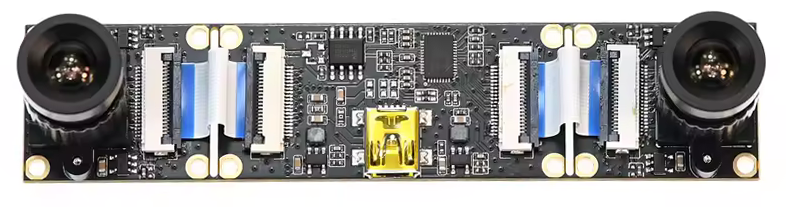
\includegraphics[width=0.5\textwidth]{images/MAINSTEREO.png}  % Adjust the path and width as necessary
    \captionsetup{font=footnotesize}
    \caption[Kamera stereowizyjna. https://cell-kom.com/inne/21454-kamera-internetowa-full-hd-b16-1080p-5900217390350.html]{Kamera stereowizyjna}
    \label{fig:mono}  % Optional: use to refer to this image later in the text
\end{figure}

Stereowizja (lub Wizja stereoskopowa) to technika polegająca na wykorzystaniu dwóch (lub więcej) obrazów tej samej sceny, uchwyconych z nieco innych punktów widzenia, do wyodrębnienia informacji przestrzennych. Jest to jedno z najstarszych i najintensywniej badanych podejść do estymacji głębi, inspirowane sposobem, w jaki ludzkie oczy – jako dwa przesunięte względem siebie punkty obserwacyjne – postrzegają świat trójwymiarowy.

W odróżnieniu od wizji monokularnej, stereowizja oferuje geometrycznie uzasadnioną możliwość bezpośredniego obliczenia głębokości, co czyni ją bardzo atrakcyjną w aplikacjach wymagających wysokiej dokładności. W tym rozdziale przedstawiono podstawy matematyczne wizji stereo, klasyczne i współczesne metody obliczania głębi, a także omówiono praktyczne zastosowania i ograniczenia tej technologii.

W systemie stereowizyjnym wykorzystuje się dwa obrazy uchwycone przez kamery umieszczone w znanej odległości od siebie (baza stereo). Podstawowym pojęciem jest paralaksa – przesunięcie obrazu tego samego punktu sceny pomiędzy obrazami lewego i prawego oka/kamery.

Zakładając idealną konfigurację (kamery wyrównane, płaszczyzny obrazu równoległe), głębokość $Z$ danego punktu sceny można obliczyć ze wzoru:
\[
z = \frac{f \cdot B}{d}
\]
\begin{itemize}
  \item $f$ - ogniskowa kamery.
  \item $B$ - odległość między kamerami.
  \item $d$ - przesunięcie danego punktu w obrazie lewym względem prawego.
\end{itemize}

Im większe $d$, tym mniejsza głębokość – obiekty bliżej kamery mają większe przesunięcie między obrazami.

\begin{minipage}[t]{\textwidth}
\textbf{Wady i ograniczenia:}
\begin{itemize}
  \item Wymóg kalibracji i synchronizacji kamer – błędy w tym zakresie przekładają się bezpośrednio na błędną głębokość.

  \item Brak dopasowania w teksturowo ubogich obszarach – np. białe ściany, niebo.

  \item Problemy przy silnym oświetleniu i odbiciach – zmienność intensywności zaburza dopasowanie.

  \item Duży koszt obliczeniowy – szczególnie w przypadku metod globalnych lub opartych na deep learningu.

  \item Widzenie tylko z jednej perspektywy – martwe strefy między kamerami lub poza polem widzenia jednej z nich.
\end{itemize}
\end{minipage}

\subsection{Structured Light}

\begin{figure}[H]  % 'h' means "here", it places the figure at the current location in the document
    \centering  % Centers the image
    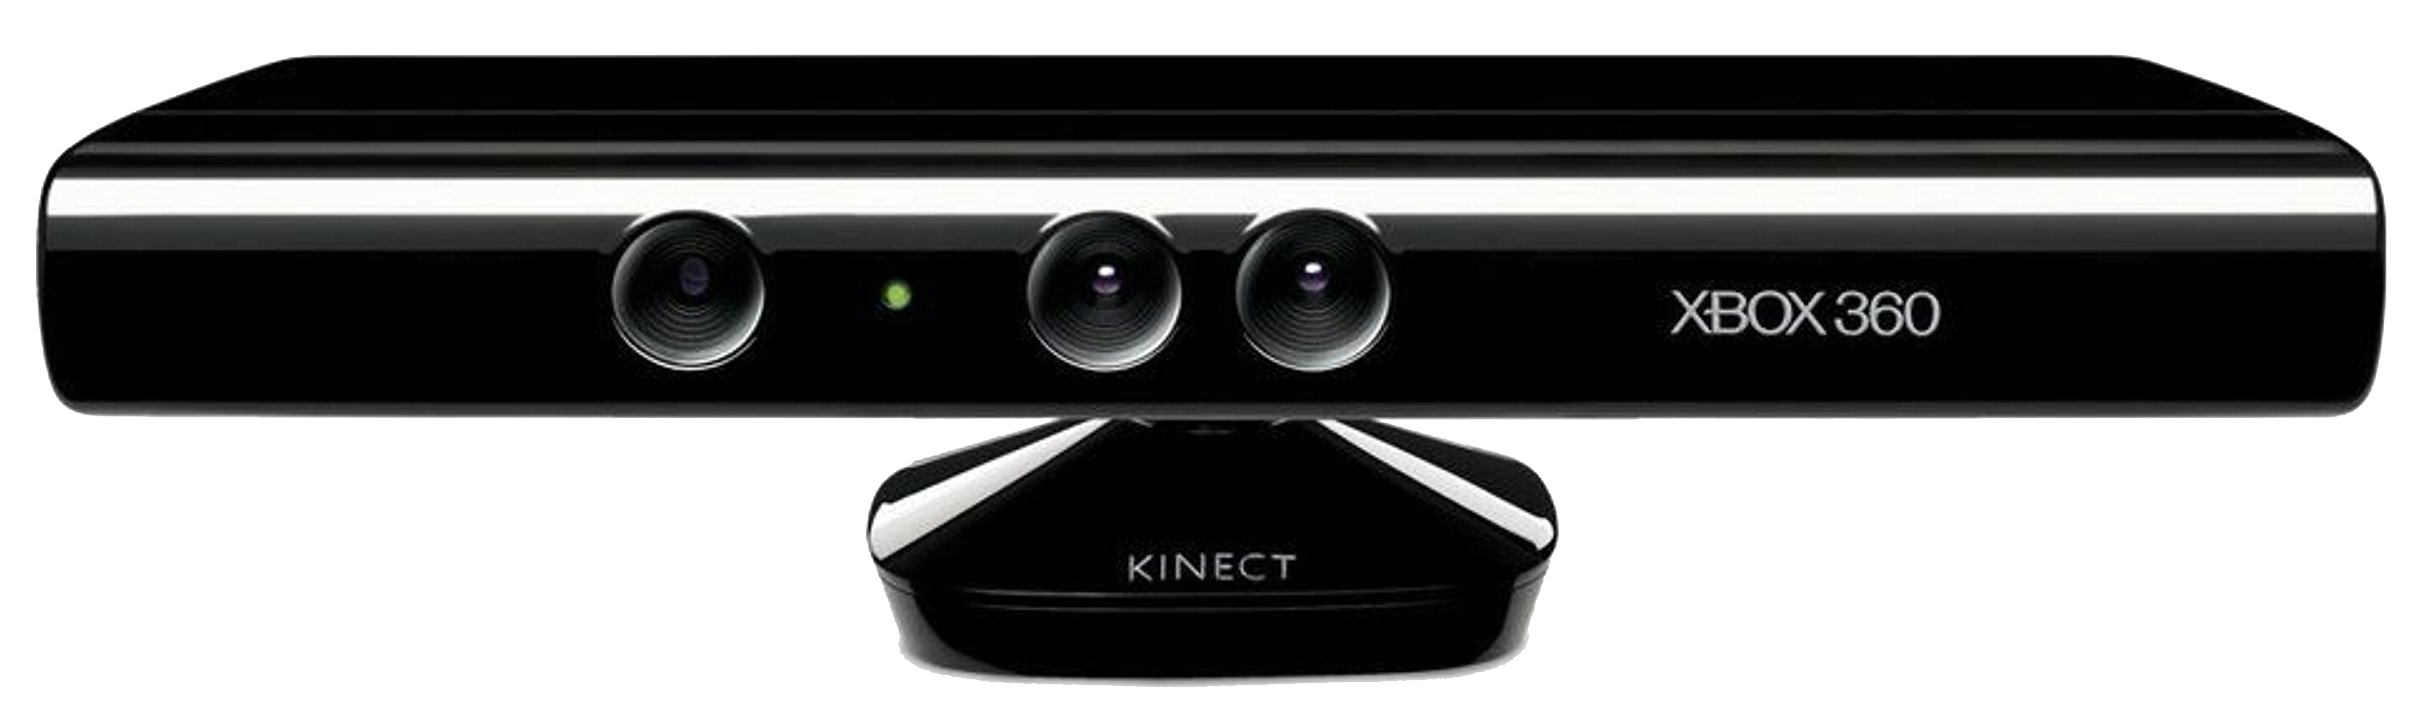
\includegraphics[width=0.5\textwidth]{images/POINTCLOUD.png}  % Adjust the path and width as necessary
    \captionsetup{font=footnotesize}
    \caption[Kamera Xbox 360 Kinect. https://cell-kom.com/inne/21454-kamera-internetowa-full-hd-b16-1080p-5900217390350.html]{Kamera Xbox 360 Kinect}
    \label{fig:kinect}  % Optional: use to refer to this image later in the text
\end{figure}

Structured Light (pol. światło strukturalne) to technika aktywnej wizji komputerowej wykorzystywana do precyzyjnego pomiaru kształtu i głębokości obiektów. Polega na projekcji znanego wzorca świetlnego (np. siatki, kropek, pasków) na powierzchnię sceny, a następnie analizie deformacji tego wzorca za pomocą kamery.

\bigskip

System Structured Light składa się zazwyczaj z dwóch komponentów:

\begin{itemize}
  \item Projektora – emituje wzorzec świetlny (np. siatkę punktów lub paski) na obserwowaną scenę.

  \item Kamery – rejestruje zniekształcony wzorzec po odbiciu od obiektów w przestrzeni.
\end{itemize}

Proces działa następująco:

\begin{enumerate}
  \item Znany wzorzec zostaje wyświetlony na scenie.

  \item Gdy wzorzec napotyka obiekty o różnych kształtach i odległościach, zostaje geometrycznie zniekształcony.

  \item Kamera rejestruje te deformacje.

  \item System porównuje zarejestrowany obraz wzorca ze wzorcem referencyjnym, który byłby widoczny na płaskiej powierzchni.

  \item Na podstawie różnic (tzw. disparity) obliczana jest głębokość – za pomocą triangulacji.
\end{enumerate}

\begin{minipage}[t]{\textwidth}
\textbf{Wady i ograniczenia:}
\begin{itemize}
  \item W jasnym świetle dziennym (szczególnie na zewnątrz), wzorzec świetlny może zostać zaburzony lub całkowicie zaniknąć – szczególnie jeśli działa w paśmie IR.

  \item Technika najlepiej sprawdza się na krótkich dystansach (0,5–2 m). Dalsze obiekty dają mniej wyraźne zniekształcenia wzorca.

  \item Szkło, lustra, woda lub powierzchnie metaliczne mogą zaburzyć wzorzec lub wprowadzać wielokrotne odbicia.

  \item Projektor i kamera muszą być precyzyjnie skalibrowane względem siebie – błędy kalibracji mogą znacząco wpłynąć na jakość głębi.

  \item Gdy wzorzec nie dotrze do części sceny (np. w załomach, pod kątem), pomiar głębokości w tych miejscach będzie niemożliwy.
\end{itemize}
\end{minipage}

\subsection{LIDAR (Light Detection and Ranging)}

\begin{figure}[H]  % 'h' means "here", it places the figure at the current location in the document
    \centering  % Centers the image
    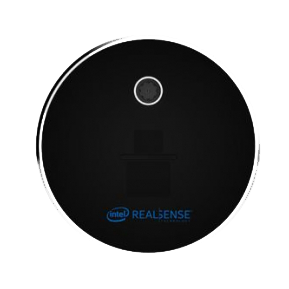
\includegraphics[width=0.3\textwidth]{images/LIDAR.png}  % Adjust the path and width as necessary
    \captionsetup{font=footnotesize}
    \caption[Kamera Intel RealSense L515 z technologią LIDAR. https://cell-kom.com/inne/21454-kamera-internetowa-full-hd-b16-1080p-5900217390350.html]{Kamera Intel RealSense z technologią LIDAR.}
    \label{fig:mono}  % Optional: use to refer to this image later in the text
\end{figure}

LIDAR (Light Detection and Ranging) to technologia zdalnego pomiaru odległości, która działa poprzez wysyłanie impulsów laserowych i mierzenie czasu, jaki upływa od ich odbicia od obiektu do powrotu do sensora. Na tej podstawie LIDAR tworzy bardzo dokładne mapy 3D otoczenia.

Podstawowy mechanizm działania LiDAR opiera się na bardzo prostej zasadzie:

\begin{itemize}
  \item Sensor emituje impuls laserowy w kierunku otoczenia.
  \item Światło odbija się od powierzchni obiektów i wraca do detektora.
  \item System mierzy czas, jaki upłynął od wysłania do odebrania sygnału (Time-of-Flight, ToF).
  \item Znając prędkość światła, obliczana jest dokładna odległość:
    \[
    d = \frac{c \cdot \Delta t}{2}
    \]

  gdzie:
  \begin{align*}
  d &- \text{odległość do obiektu} \\
  c &- \text{prędkość światła (ok. } 3 \cdot 10^8 \, \text{m/s)} \\
  \Delta t &- \text{czas przelotu sygnału}
  \end{align*} 
\end{itemize}

LiDAR-y mogą wykonywać takie pomiary miliony razy na sekundę, skanując środowisko w 2D (jeden plan) lub 3D (pełna chmura punktów).

\begin{minipage}[t]{\textwidth}
\textbf{Wady i ograniczenia:}
\begin{itemize}
  \item Mgła, deszcz, śnieg i kurz mogą zakłócać odbicie promieni lasera, co wpływa na dokładność pomiarów.

  \item Brak dopasowania w teksturowo ubogich obszarach – np. białe ściany, niebo.

  \item LiDAR rejestruje wyłącznie dane geometryczne – nie dostarcza żadnych informacji o kolorze czy teksturze powierzchni.

  \item W porównaniu do kamer, LiDAR-y mają stosunkowo rzadką siatkę pomiarową, co skutkuje niższą rozdzielczością przy dużych odległościach (np. obiekt 100 m dalej może być opisany przez kilka punktów).

  \item Bardzo ciemne lub przezroczyste powierzchnie (np. szyby) mogą słabo odbijać impulsy lasera lub w ogóle je przepuszczać.
\end{itemize}
\end{minipage}

\subsection{Kamery zdarzeniowe}

Kamery zdarzeniowe (ang. Event Cameras) to innowacyjne sensory wizyjne, które różnią się fundamentalnie od tradycyjnych kamer opartych na matrycy CMOS. Zamiast przechwytywać obraz w sposób klatkowy (frame-based), rejestrują one zmiany jasności na poziomie pojedynczych pikseli, co pozwala na znacznie wyższą rozdzielczość czasową i lepszą reakcję na dynamiczne sceny. Dzięki temu technologia ta znajduje coraz szersze zastosowanie w systemach robotycznych, autonomicznych pojazdach, AR/VR i przetwarzaniu sygnałów w czasie rzeczywistym.

W tradycyjnych kamerach każda klatka rejestrowana jest w określonym interwale czasowym, co powoduje powstawanie rozmycia ruchu i dużego opóźnienia w dynamicznych scenach. Kamery zdarzeniowe działają zupełnie inaczej:

Każdy piksel działa niezależnie i stale monitoruje zmiany lokalnej jasności.

Gdy zmiana przekroczy ustalony próg (np. 10% zmiany jasności), piksel generuje tzw. zdarzenie (event).

Zdarzenie zawiera informację o:

\begin{itemize}
  \item położeniu piksela (x, y),

  \item czasie zdarzenia (z dokładnością do mikrosekund),

  \item polaryzacji zmiany (jasność wzrosła lub zmalała).
\end{itemize}

Dzięki temu kamera generuje strumień asynchronicznych zdarzeń, a nie szereg klatek. Przykładami takich kamer są m.in. DVS (Dynamic Vision Sensor), DAVIS (łączący klasyczną kamerę z kamerą zdarzeniową) oraz CeleX.

Brak informacji o statycznych obiektach: jeśli scena się nie zmienia, kamera nie generuje zdarzeń – co utrudnia pełną rekonstrukcję otoczenia.

Trudności w przetwarzaniu danych: strumień zdarzeń ma inną strukturę niż klasyczne obrazy – wymaga specjalnych algorytmów i często dedykowanego sprzętu (np. FPGA).

Niska rozdzielczość przestrzenna: w porównaniu do tradycyjnych kamer, choć technologia ta dynamicznie się rozwija.

Szum przy słabym oświetleniu: niektóre sensory są bardziej podatne na fałszywe zdarzenia w nocy lub w ciemnych pomieszczeniach.

Koszt: kamery zdarzeniowe są wciąż relatywnie drogie i mniej dostępne komercyjnie.

\begin{minipage}[t]{\textwidth}
\textbf{Wady i ograniczenia:}
\begin{itemize}
  \item Wymóg kalibracji i synchronizacji kamer – błędy w tym zakresie przekładają się bezpośrednio na błędną głębokość.

  \item Brak dopasowania w teksturowo ubogich obszarach – np. białe ściany, niebo.

  \item Problemy przy silnym oświetleniu i odbiciach – zmienność intensywności zaburza dopasowanie.

  \item Duży koszt obliczeniowy – szczególnie w przypadku metod globalnych lub opartych na deep learningu.

  \item Widzenie tylko z jednej perspektywy – martwe strefy między kamerami lub poza polem widzenia jednej z nich.
\end{itemize}
\end{minipage}



\section{Opis projektu}

\begin{figure}[H]  % 'h' means "here", it places the figure at the current location in the document
    \centering  % Centers the image
    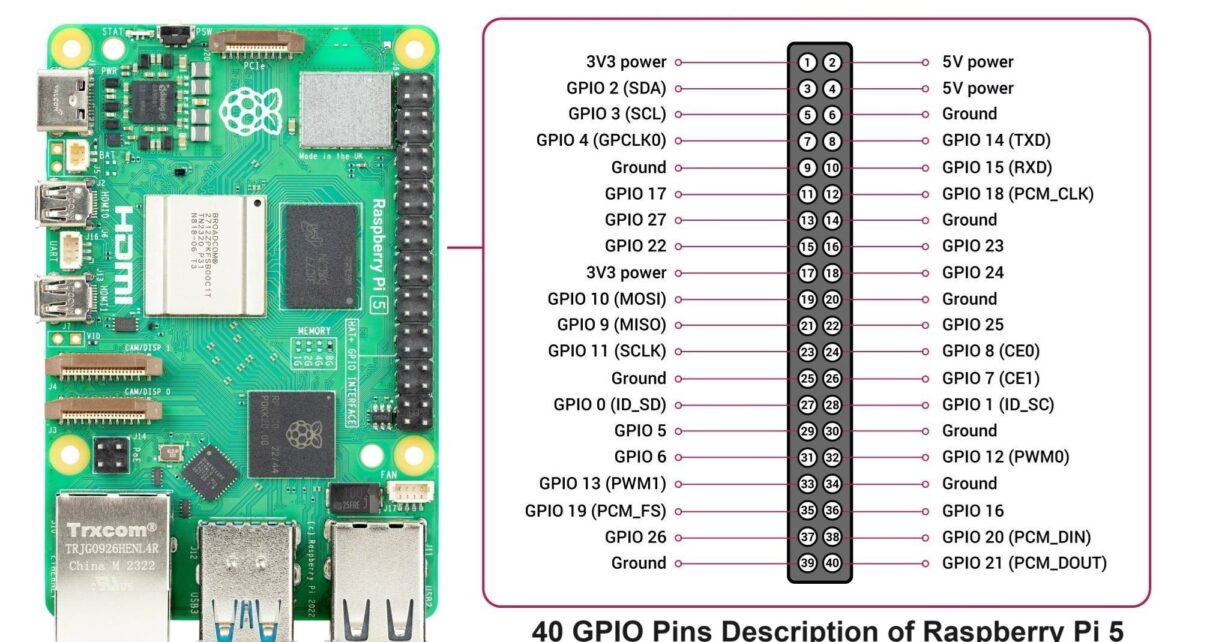
\includegraphics[width=0.6\textwidth]{images/RPI-PIN.jpg}  % Adjust the path and width as necessary
    \captionsetup{font=footnotesize}
    \caption[Płytka Raspberry Pi 5 i jej schemat pinów GPIO. https://www.hackatronic.com/wp-content/uploads/2024/03/Raspberry-Pi-5-Pinout--1210x642.jpg]{Płytka Raspberry Pi 5 i jej schemat pinów GPIO.}
\end{figure}

\begin{figure}[H]  % 'h' means "here", it places the figure at the current location in the document
    \centering  % Centers the image
    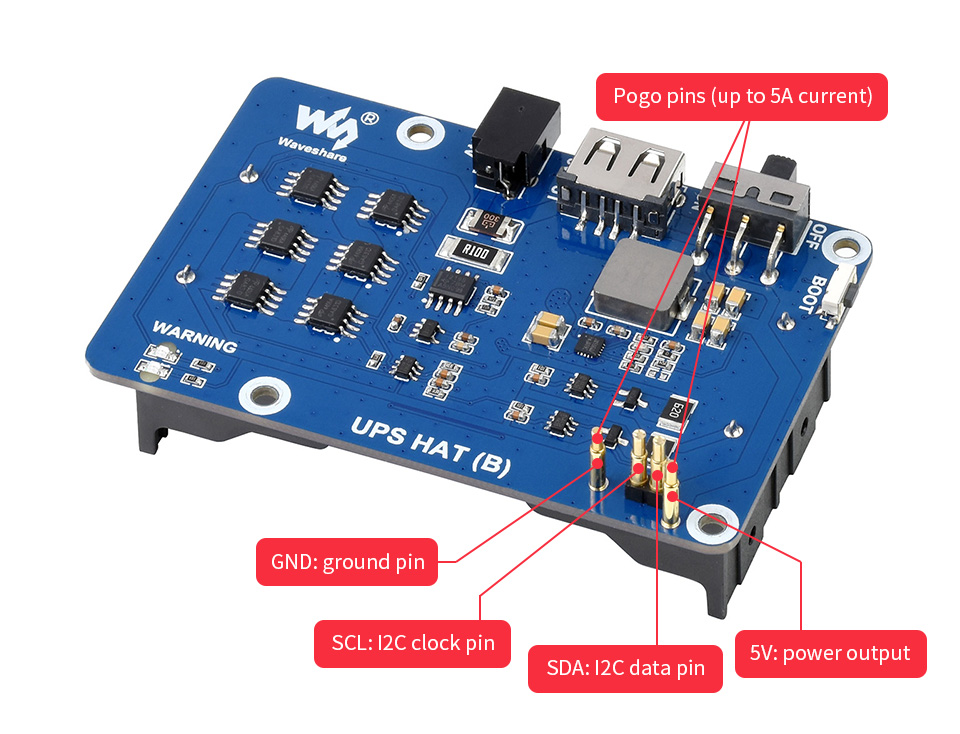
\includegraphics[width=0.6\textwidth]{images/ups-hat.jpg}  % Adjust the path and width as necessary
    \captionsetup{font=footnotesize}
    \caption[Moduł zasilający. https://www.waveshare.com/wiki/UPS-HAT-(B)]{Moduł zasilający.}
\end{figure}

Umowżliwia bezpośrednie podpięcie zasilania pod Raspberry Pi (3/4/5) poprzez Pogo piny, nie wykorzystując GPIO.

Moduł posiada również: ochronę przed przeładowaniem, nadmiernym rozładowaniem, zbyt dużym poborem prądu, zwarciem oraz odwrotną polaryzacją

\textbf{Napięcie wyjściowe:} 5~V \\
\textbf{Maksymalny prąd wyjściowy:} do 5~A \\
\textbf{Obsługiwane ogniwa:} 2 × akumulatory 18650, 3{,}7~V (7{,}4~V nominalnie)

\textbf{Obliczenia czasu pracy dwóch akumulatorów 18650}

\textbf{Dane:}
\begin{itemize}
  \item Napięcie nominalne akumulatora: $U = 3{,}7\,\mathrm{V}$
  \item Pojemność jednego akumulatora: $C = 8800\,\mathrm{mAh} = 8{,}8\,\mathrm{Ah}$
  \item Ilość akumulatorów: 2 (założenie: połączone równolegle lub przez przetwornicę)
  \item Całkowita pojemność: $C_{\text{total}} = 2 \cdot 8{,}8 = 17{,}6\,\mathrm{Ah}$
  \item Maksymalny pobór prądu przez urządzenie: $I = 5\,\mathrm{A}$
  \item Napięcie wyjściowe: $U_{\text{out}} = 5\,\mathrm{V}$
  \item Sprawność przetwornicy (założenie): $\eta = 0{,}85$ (czyli 85\%)
\end{itemize}

\textbf{Krok 1: Obliczenie energii dostępnej z akumulatorów:}

\[
E = U \cdot C_{\text{total}} = 3{,}7\,\mathrm{V} \cdot 17{,}6\,\mathrm{Ah} = 65{,}12\,\mathrm{Wh}
\]

\textbf{Krok 2: Obliczenie mocy pobieranej przez urządzenie:}

\[
P = U_{\text{out}} \cdot I = 5\,\mathrm{V} \cdot 5\,\mathrm{A} = 25\,\mathrm{W}
\]

\textbf{Krok 3: Uwzględnienie sprawności przetwornicy:}

\[
P_{\text{real}} = \frac{P}{\eta} = \frac{25\,\mathrm{W}}{0{,}85} \approx 29{,}41\,\mathrm{W}
\]

\textbf{Krok 4: Obliczenie czasu pracy:}

\[
t = \frac{E}{P_{\text{real}}} = \frac{65{,}12\,\mathrm{Wh}}{29{,}41\,\mathrm{W}} \approx 2{,}21\,\mathrm{h}
\]

\textbf{Odpowiedź:} Przy maksymalnym poborze prądu $5\,\mathrm{A}$ moduł będzie działać około $2{,}2$ godziny.

\begin{figure}[H]  % 'h' means "here", it places the figure at the current location in the document
    \centering  % Centers the image
    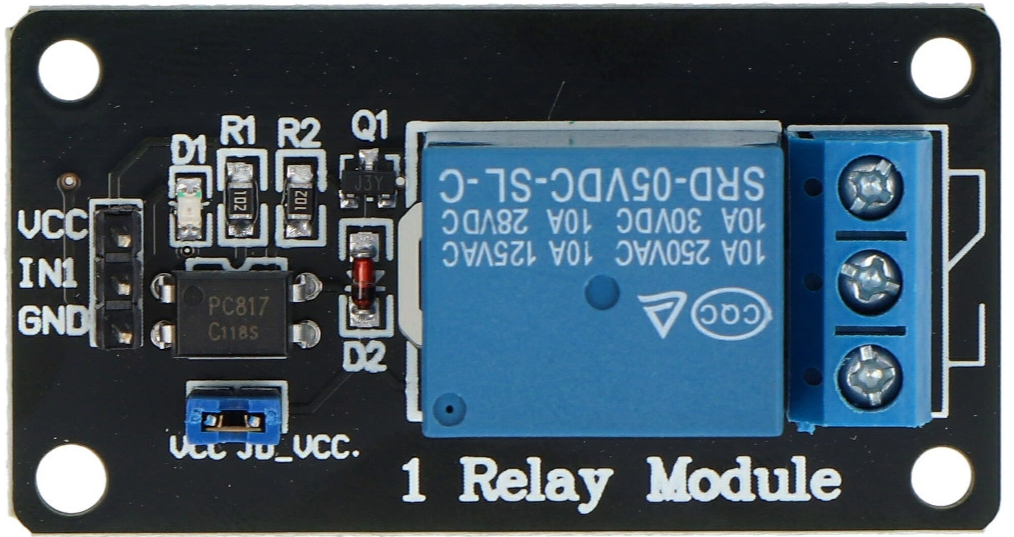
\includegraphics[width=0.4\textwidth]{images/relay.png}  % Adjust the path and width as necessary
    \captionsetup{font=footnotesize}
    \caption[Moduł przekaźnika. https://botland.com.pl/przekazniki-przekazniki-arduino/1997-modul-przekaznika-1-kanal-z-optoizolacja-styki-10a-250vac-cewka-5v-5904422359096.html]{Moduł przekaźnika.}
\end{figure}

Układ pozwala na sterowanie elementami wykonawczymi przy pomocy portów mikrokontrolera lub dowolnego zestawu uruchomieniowego.

\section{Obrazowanie stereoskopowe}

Stereo Vision umożliwia rozpoznawanie głębi na obrazie, wykonywanie pomiarów na obrazie
i przeprowadzanie lokalizacji 3D. Między innymi należy znaleźć punkty, które pasują do siebie między dwiema kamerami. Można to następnie wykorzystać do odległość między kamerą a punktem. Wykorzystywana jest geometria systemu w celu uproszczenia obliczeń.

Te cztery kroki są wykonywane podczas obrazowania stereo:

\begin{enumerate}
  \item usuwanie zniekształceń promieniowych i stycznych za pomocą obliczeń matematycznych
obliczenia. W ten sposób powstają obrazy bez deformacji.
  \item rektyfikacja kąta i odległości obrazów. Na tym etapie oba obrazy są
obrazy współpłaszczyznowe na osi $Y$, co ułatwia wyszukiwanie korespondencji.
łatwiejsze i wystarczy szukać tylko na jednej osi (osi $X$).
  \item znajdź tę samą cechę na prawym i lewym obrazie. Daje to mapę dysproporcji pokazującą różnice między obrazami na osi $X$.
  \item Ostatnim krokiem jest triangulacja. Mapa rozbieżności jest przekształcana w odległości za pomocą triangulacji.
\end{enumerate}

\subsection{Triangulacja}

\begin{figure}[H]  % 'h' means "here", it places the figure at the current location in the document
    \centering  % Centers the image
    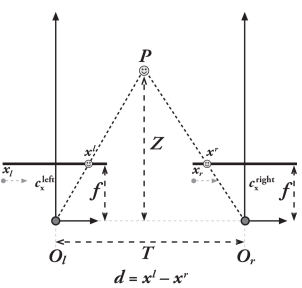
\includegraphics[width=0.5\textwidth]{images/triangulation.png}  % Adjust the path and width as necessary
    \captionsetup{font=footnotesize}
    \caption[Schemat triangulacji. Learning OpenCV 3, O'Reilly, Str. 705]{Schemat triangulacji.}
    \label{fig:rpi}  % Optional: use to refer to this image later in the text
\end{figure}

W ostatnim kroku, triangulacji, zakłada się, że oba obrazy projekcji są współpłaszczyznowe i że poziomy rząd pikseli lewego obrazu jest wyrównany z odpowiadającym mu obrazem prawego.

Poniższy obraz można teraz skonstruować przy użyciu poprzednich hipotez.

Punkt $P$ leży w środowisku i jest pokazany na
lewym i prawym obrazie na $P_l$ i $P_r$, z odpowiadającymi im współrzędnymi
odpowiadającymi współrzędnymi $X_l$ i $X_r$. To pozwala nam wprowadzić nową wielkość $d = X_l - X_r$.
Można zauważyć, że im dalej punkt $P$, tym mniejsza staje się wielkość $d$. Dysproporcja jest zatem odwrotnie proporcjonalna do odległości.\\
Do obliczenia odległości można użyć następującego wzoru można obliczyć: \[Z=f*T/(xl-xr)\]

Można zauważyć, że istnieje nieliniowa zależność między rozbieżnością a odległością.
Jeśli rozbieżność jest bliska 0, małe różnice w rozbieżności prowadzą do dużych różnic w odległości.
Zjawisko to ulega odwróceniu, gdy rozbieżność jest duża. Małe różnice dysproporcji nie prowadzą do dużych różnic odległości. Na tej podstawie można wywnioskować, że stereowizja ma wysoką rozdzielczość głębi, tylko dla obiektów znajdujących się blisko kamery.

Metoda ta działa jednak tylko wtedy, gdy konfiguracja kamery stereo jest idealna. W
rzeczywistości tak nie jest. Właśnie dlatego lewy i prawy obraz są
matematycznie wyrównane równolegle. Oczywiście kamery muszą być fizycznie ustawione równolegle.
Zanim zostanie wyjaśniona metoda matematycznego wyrównywania obrazów, trzeba najpierw zrozumieć geometrię epipolarną.

\subsection{Geometria epipolarna}

\begin{figure}[H]  % 'h' means "here", it places the figure at the current location in the document
    \centering  % Centers the image
    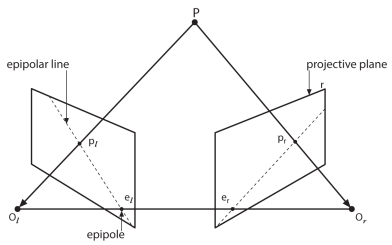
\includegraphics[width=0.5\textwidth]{images/epipolar.png}  % Adjust the path and width as necessary
    \captionsetup{font=footnotesize}
    \caption[Model kamery stereo. Learning OpenCV 3, O'Reilly, Str. 709]{Model kamery stereo.}
    \label{fig:rpi}  % Optional: use to refer to this image later in the text
\end{figure}

Powyższy obrazek przedstawia model niedoskonałej kamery stereo składającej się z dwóch modeli kamer otworkowych.
Przecięcie linii środków projekcji ($O_l$, $O_r$) z płaszczyznami projekcji tworzone są punkty epipolarne $e_l$ i $e_r$. Linie ($p_l$, $e_l$) i ($p_r$, $e_r$) są nazywane liniami epipolarnymi. Obrazem wszystkich możliwych punktów punktu
na płaszczyźnie rzutowania jest linia epipolarna, która leży na drugiej płaszczyźnie obrazu i
przechodzi przez punkt epipolarny i szukany punkt. Umożliwia to ograniczenie wyszukiwania punktu na jednym wymiarze zamiast na całej płaszczyźnie.\\
Można zatem podsumować następujące punkty:

\begin{itemize}
  \item Każdy punkt 3D w widoku kamery jest zawarty w planie epipolarnym
  \item Element w jednej płaszczyźnie musi znajdować się na odpowiednich liniach epipolarnych drugiej płaszczyzny (warunek epipolarny).
drugiej płaszczyzny (warunek epipolarny)
  \item Dwuwymiarowe wyszukiwanie odpowiadającego elementu jest konwertowane na
jednowymiarowe, jeśli znana jest geometria epipolarna.
  \item Kolejność punktów jest zachowana, tzn. dwa punkty $A$ i $B$ są w tej samej kolejności na liniach epipolarnych płaszczyzny.

\end{itemize}

ta sama kolejność na liniach epipolarnych jednej płaszczyzny, co na liniach epipolarnych drugiej płaszczyzny.

\subsection{Macierze podstawowe i fundamentalne}

Aby zrozumieć, w jaki sposób obliczane są linie epipolarne, musimy najpierw wyjaśnić macierze podstawowe
i macierze fundamentalne (odpowiadające macierzom $E$ i $F$).
Macierz podstawowa $E$ zawiera informacje o tym, jak fizycznie rozmieszczone są obie kamery.
Opisuje ona lokalizację drugiej kamery względem pierwszej za pomocą parametrów translacji i rotacji.
Parametrów tych nie można odczytać bezpośrednio w macierzy, ponieważ jest ona używana do planowania projektu. W sekcji Kalibracja stereo wyjaśnone będzie, jak obliczyć $R$ i $T$ (macierz rotacji i wektor translacji).
Macierz $F$ zawiera informacje z podstawowej macierzy $E$, fizyczny układ kamer i informacje o wewnętrznych parametrach kamer.
Relacja między rzutowanym punktem na lewym obrazie $p_l$ i rzutowanym punktem na prawym obrazie $p_r$ jest zdefiniowana następująco:

\[prTEpl=0\]
Można by pomyśleć, że ta formuła w pełni opisuje związek między lewym i prawym punktem.
prawym punktem. Należy jednak zauważyć, że macierz 3x3 $E$ jest rzędu
jest rangi 2. Oznacza to, że wzór ten jest równaniem prostej.
Aby w pełni zdefiniować relację między punktami, parametry wewnętrzne.
parametry wewnętrzne.
Pamiętamy, że $q = Mp$, z macierzą wewnętrzną $M$.
Podstawienie do poprzedniego równania daje wynik:
\[qrT(Ml-1)TEMl-1ql=0\]
Podstawienie:\\
\[F=(Ml-1)TEMl-1\]
W ten sposób otrzymujemy\\
\[qrTFql=0\]

\subsection{Macierz obrotu i wektor przesunięcia}

Teraz, gdy zostałą wyjaśniona macierz podstawową $E$ i macierz podstawową $F$, trzeba zobaczyć, jak obliczyć macierz obrotu i wektor translacji.
Zdefiniujemy następujące oznaczenia:

\begin{itemize}
  \item $P_l$ i $P_r$ definiują pozycje punktu w układzie współrzędnych odpowiednio lewej i prawej kamery.
  \item $R_l$ i $T_l$ (lub $R_r$ i $T_r$) definiują obrót i translację z kamery
do punktu w otoczeniu dla lewej (lub prawej) kamery.
  \item $R$ i $T$ to obrót i translacja układu współrzędnych prawej kamery w układzie współrzędnych lewej kamery.
\end{itemize}

Daje to następujące wyniki
\[
\begin{array}{cc}
P_l = R_l P + T_l & \quad P_r = R_r P + T_r
\end{array}
\]
Mamy również:
\[Pl=RT(Pr-T)\]
Z tych trzech równań ostateczny wynik to
\[
\begin{array}{cc}
R = R_r R_l^T & \quad T = T_r - R T_l
\end{array}
\]

\subsection{Rektyfikacja stereo}

Zadaniem rektyfikacji jest rzutowanie dwóch obrazów tak, aby leżały dokładnie w tej samej płaszczyźnie i precyzyjne wyrównanie rzędów pikseli tak, aby linie epipolarne stały się poziome w celu zapewnienia zgodności punktu na dwóch obrazach.
aby znaleźć zgodność punktu na dwóch obrazach w sposób bardziej losowy.
W wyniku procesu wyrównywania obu obrazów uzyskuje się 8 wyrażeń, po 4 dla każdej kamery:

\begin{itemize}
  \item wektor zniekształceń
  \item macierz rotacji Rrect, która musi zostać zastosowana do obrazu
  \item wyprostowana macierz kamery Mrect
  \item nierektyfikowana macierz kamery $M$
\end{itemize}

OpenCV pozwala nam obliczyć te warunki za pomocą dwóch algorytmów: algorytmu Hartley'a
i algorytmu Bouguet'a.

\subsubsection{Algorytm Hartley'a}

Algorytm Hartley’a jest metodą rektyfikacji niekalibrowanej, czyli nie wymaga znajomości parametrów wewnętrznych kamer (np. ogniskowej, współrzędnych środka obrazu, współczynników zniekształceń soczewek). Jest to istotne w zastosowaniach, gdzie dostępne są tylko obrazy, bez wcześniejszej kalibracji sprzętu.

\bigskip

Kluczowe kroki:

\begin{itemize}
\item Najpierw algorytm odnajduje zestawy punktów, które występują na obu obrazach — tzw. korespondencje punktowe. W praktyce mogą to być np. punkty narożne, cechy SIFT, SURF czy ORB.

\item Z punktów odpowiadających estymowana jest macierz fundamentalna, która opisuje geometryczne powiązania pomiędzy dwoma obrazami.

\item Za pomocą macierzy F obliczane są transformacje projekcyjne (homografie) dla obu obrazów, które przekształcają je w taki sposób, aby epipole zostały przekształcone w nieskończoność, co oznacza, że linie epipolowe stają się poziome i równoległe.

Dzięki temu poszukiwanie dopasowań między obrazami można sprowadzić do jednej osi (najczęściej poziomej), co znacząco upraszcza dalszą analizę.
\end{itemize}

Główną wadą tej metody jest jednak to, że nie dostarcza informacji o rzeczywistej skali sceny. Oznacza to, że uzyskane dane dotyczą jedynie względnego położenia obiektów, bez możliwości dokładnego określenia ich odległości od kamery. W rezultacie, mimo że algorytm umożliwia uzyskanie rektyfikowanych obrazów, jego precyzja jest niższa w porównaniu do metod opartych na pełnej kalibracji kamer.

\subsubsection{Algorytm Bouguet'a}

Algorytm Bouguet’a (opracowany m.in. w ramach narzędzia Camera Calibration Toolbox do MATLABa) to metoda rektyfikacji kalibrowanej, czyli wykorzystująca uprzednio wyznaczone parametry wewnętrzne i zewnętrzne kamer.

\bigskip

Kluczowe kroki:

\begin{itemize}
  \item Na podstawie obrazów wzorca (np. szachownicy) określane są parametry wewnętrzne każdej kamery (ogniskowa, środek obrazu, zniekształcenia) oraz parametry zewnętrzne (rotacja i translacja między kamerami).

  \item Obrazy są odwzorowywane do wspólnej przestrzeni trójwymiarowej, w której określona jest pozycja i orientacja obu kamer.


  \item Płaszczyzny obrazów są obracane w taki sposób, by ich główne osie optyczne stały się równoległe (tzn. skierowane w tym samym kierunku), a obrazy znajdowały się w tej samej płaszczyźnie. Dzięki temu linie epipolowe stają się poziome i równoległe — jak w przypadku metody Hartley’a, ale z większą precyzją.


  \item Na podstawie wyliczonych rzutów generowane są nowe obrazy zrektyfikowane, w których każdy piksel z jednej kamery można bezpośrednio porównać z pikselem z drugiej kamery w tej samej linii poziomej.
\end{itemize}

Algorytm Bouguet’a wymaga wcześniejszej kalibracji kamer, co wiąże się z koniecznością poświęcenia dodatkowego czasu oraz użycia odpowiednich narzędzi, takich jak wzorce kalibracyjne (np. szachownica) i oprogramowanie do analizy obrazów. Choć taka kalibracja pozwala uzyskać bardzo precyzyjne wyniki, metoda ta jest wrażliwa na błędy kalibracji — na przykład niedokładne wykrycie wzorca kalibracyjnego lub jego niewłaściwe ujęcie na zdjęciach może znacząco pogorszyć jakość rektyfikacji, prowadząc do błędów w dalszym przetwarzaniu obrazów.

\chapter{Rozdział badawczy}

\section{Funkcjonalność programu do obrazowania stereo}

Jak już wspomniano, program jest kodowany w Pythonie i wykorzystywana jest biblioteka OpenCV.
jest używana. Zdecydowaliśmy się na język Python i bibliotekę OpenCV, ponieważ
mieliśmy już z nimi doświadczenie i ponieważ istnieje wiele dokumentacji na ich temat. Innym
argumentem za tą decyzją jest to, że chcieliśmy pracować tylko z bibliotekami „open source”.
biblioteki.
Na potrzeby tego projektu opracowano dwa programy w języku Python.
Pierwszy z nich, „Take-images-for-calibration.py”, służy do robienia dobrych zdjęć, które są później wykorzystywane do kalibracji obu kamer.
Później są one wykorzystywane do kalibracji obu kamer (kalibracja zniekształceń i kalibracja stereo).
kalibracja.
Drugi program, a tym samym główny program „Main-Stereo-Vision-Prog.py” jest używany do obrazowania stereo.
jest używany do obrazowania stereo. W tym programie kalibrujemy kamery za pomocą wykonanych zdjęć, generujemy mapę dysproporcji i dzięki doświadczalnemu równaniu
równania, które zostało znalezione eksperymentalnie, możemy zmierzyć odległość dla każdego piksela.
pomiar. Na końcu używany jest filtr WLS, aby lepiej rozpoznawać krawędzie obiektów.
rozpoznać krawędzie obiektów.

Po uruchomieniu tego programu obie kamery stają się aktywne i otwierane są dwa okna.
aby użytkownik mógł zobaczyć, gdzie na obrazach znajduje się szachownica.


\subsection{Kalibracja}

\begin{lstlisting}[style=mypython]
# Termination criteria
criteria =(cv2.TERM_CRITERIA_EPS + cv2.TERM_CRITERIA_MAX_ITER, 30, 0.001)
criteria_stereo= (cv2.TERM_CRITERIA_EPS + cv2.TERM_CRITERIA_MAX_ITER, 30, 0.001)

# Przygotowanie punktow obiektu
objp = np.zeros((9*6,3), np.float32)
objp[:,:2] = np.mgrid[0:9,0:6].T.reshape(-1,2)

# Tablice do przechowywania punktow obiektu i punktow obrazu ze wszystkich obrazow
objpoints= []   # Punkty 3D w przestrzeni swiata rzeczywistego
imgpointsR= []   # Punkty 2D na plaszczyznie obrazu
imgpointsL= []

for i in range(0, 64):
    t = str(i)
    ChessImgR = cv2.imread('calib_images/right_chessboard-' + t + '.png', 0)
    ChessImgL = cv2.imread('calib_images/left_chessboard-' + t + '.png', 0)
    if ChessImgR is None or ChessImgL is None:
        continue  # Skip this iteration if loading failed
    retR, cornersR = cv2.findChessboardCorners(ChessImgR, (9, 6), None)
    retL, cornersL = cv2.findChessboardCorners(ChessImgL, (9, 6), None)
    if retR and retL:
        objpoints.append(objp)
        cv2.cornerSubPix(ChessImgR, cornersR, (11, 11), (-1, -1), criteria)
        cv2.cornerSubPix(ChessImgL, cornersL, (11, 11), (-1, -1), criteria)
        imgpointsR.append(cornersR)
        imgpointsL.append(cornersL)

# Kalibracja
retR, mtxR, distR, rvecsR, tvecsR = cv2.calibrateCamera(objpoints, imgpointsR,
                                                        ChessImgR.shape[::-1], None, None)
retL, mtxL, distL, rvecsL, tvecsL = cv2.calibrateCamera(objpoints, imgpointsL, 
                                                        ChessImgL.shape[::-1], None, None)
OmtxR, roiR = cv2.getOptimalNewCameraMatrix(mtxR, distR, 
                                            ChessImgR.shape[::-1], 1, ChessImgR.shape[::-1])
OmtxL, roiL = cv2.getOptimalNewCameraMatrix(mtxL, distL, 
                                            ChessImgL.shape[::-1], 1, ChessImgL.shape[::-1])
\end{lstlisting}

Biblioteka OpenCV pozwala nam obliczyć parametry wewnętrzne za pomocą określonych funkcji.
Proces ten nazywany jest kalibracją. Jest to możliwe dzięki zdjęciom szachownicy wykonanym pod różnymi kątami.

Można rozpoznać dobre obrazy, na których narożniki są bardzo wyraźnie rozpoznawalne za pomocą funkcji cv2.findChesssboardCorners(). OpenCV zaleca posiadanie co najmniej 10
zdjęcia dla każdej kamery, aby uzyskać dobrą kalibrację. Do projektu zostało pobrane 32 zdjęcia dla każdej kamery.

Pozycja narożników dla każdego obrazu jest następnie zapisywana w wektorze obrazu, a punkty obiektu dla sceny 3D są zapisywane w innym wektorze. Następnie należy użyć Imgpoints i Objpoints w funkcji cv2.calibrateCamera(), której wynikiem jest macierz kamery, współczynniki zniekształceń, wektory obrotu i translacji.

Funkcja cv2.getOptimalNewCameraMatrix() umożliwia uzyskanie dokładnych macierzy kamer, które później będą wykorzystane w rektyfikacji.

Do korekcji dystorsji kamer używane są obrazy zarejestrowane za pomocą programu „calibration.py”, gdzie w zmiennych imgpoints i objpoints zapisywane są pozycje narożników szachownicy.

\begin{figure}[H]  % 'h' means "here", it places the figure at the current location in the document
    \centering  % Centers the image
    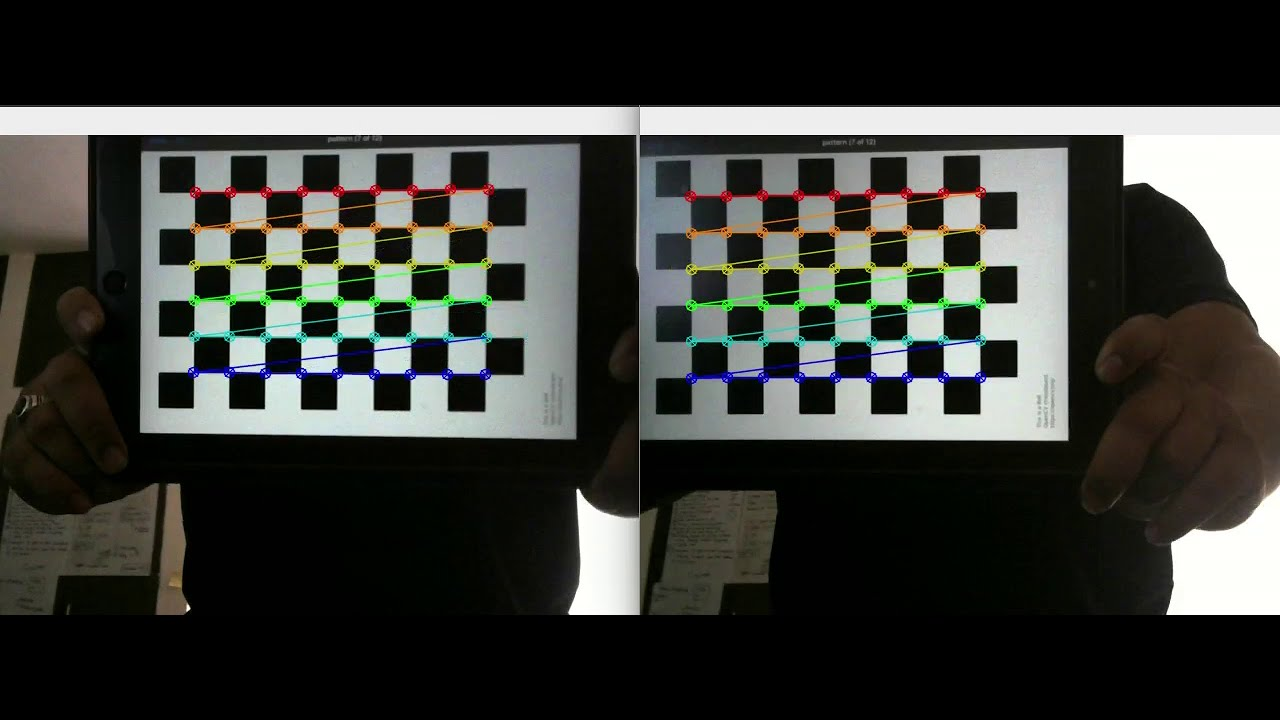
\includegraphics[width=0.8\textwidth]{images/calib.jpg}  % Adjust the path and width as necessary
    \captionsetup{font=footnotesize}
    \caption[Widok wykrytych wierzchołków szachownic. https://learnopencv.com/making-a-low-cost-stereo-camera-using-opencv/.]{Widok wykrytych wierzchołków szachownic.}
\end{figure}

Funkcja cv2.calibrateCamera() jest wykorzystywana do uzyskania nowych macierzy kamer (macierz kamery opisuje projekcję punktu ze świata 3D na obraz 2D), współczynników dystorsji, wektorów rotacji oraz translacji dla każdej z kamer. Dane te są później używane do usunięcia zniekształceń dla każdej kamery.

Aby uzyskać optymalne macierze kamer dla każdej z nich, używana jest funkcja cv2.getOptimalNewCameraMatrix() (w celu zwiększenia precyzji).

Do kalibracji stereo używana jest funkcja cv2.StereoCalibrate(), która oblicza transformację pomiędzy dwiema kamerami (jedna kamera służy jako odniesienie dla drugiej).

Po kalibracji otrzymywana jest następującą macierz $M$ dla użytej kamery:\\

Matryca $M$ bez rektyfikacji (prawa kamera):

Matrix $M_{rekt}$ Rectified (prawa kamera):

Matryca $M$ bez rektyfikacji (lewa kamera):

Matryca $M$ wyprostowana (lewa kamera):

Funkcja cv2.findChessboardCorners() wyszuka określoną liczbę narożników szachownicy
i wygenerowane zostaną następujące wektory:

\begin{itemize}
  \item imgpointsR: zawiera współrzędne narożników na prawym obrazie (w przestrzeni obrazu)
  \item imgpointsL: zawiera współrzędne narożników na lewym obrazie (w przestrzeni obrazu)
  \item objpoints: zawiera współrzędne narożników w przestrzeni obiektu.
\end{itemize}

Precyzja współrzędnych znalezionych narożników jest zwiększana za pomocą funkcji
cv2.cornerSubPix().

\subsection{Rektyfikacja}

Funkcja cv2.stereoRectify() umożliwia sprowadzenie linii epipolarnych obu kamer do tej samej płaszczyzny. Taka transformacja ułatwia działanie funkcji generującej mapę dysparycji, ponieważ dopasowywanie bloków musi być wtedy wykonywane tylko w jednym wymiarze.

Za pomocą tej funkcji uzyskuje się również macierz esencjalną oraz macierz fundamentalną, które są wykorzystywane w kolejnej funkcji.

Funkcja cv2.initUndistortRectifyMap() generuje obraz bez zniekształceń (dystorsji). Obrazy te są następnie wykorzystywane przy obliczaniu mapy dysparycji.

\begin{lstlisting}[style=mypython]
# StereoRectify function
RL, RR, PL, PR, Q, roiL, roiR= cv2.stereoRectify(MLS, dLS, MRS, dRS, ChessImgR.shape[::-1], R, T, 0,(0,0))  # last paramater is alpha, if 0= croped, if 1= not croped
# initUndistortRectifyMap function
Left_Stereo_Map= cv2.initUndistortRectifyMap(MLS, dLS, RL, PL, ChessImgR.shape[::-1], cv2.CV_16SC2)   # cv2.CV_16SC2 this format enables us the programme to work faster
Right_Stereo_Map= cv2.initUndistortRectifyMap(MRS, dRS, RR, PR, ChessImgR.shape[::-1], cv2.CV_16SC2)
\end{lstlisting}

\subsection{Mapa rozbieżności}

\begin{lstlisting}[style=mypython]
# Create StereoSGBM and prepare all parameters
block_size = 7
min_disp = 2
num_disp = 130-min_disp
stereo = cv2.StereoSGBM_create(minDisparity = min_disp,numDisparities = num_disp,blockSize = block_size,uniquenessRatio = 10,speckleWindowSize = 100,speckleRange = 32, disp12MaxDiff = 5,
    P1 = 8*3*block_size**2,
    P2 = 32*3*block_size**2)

# Used for the filtered image
stereoR=cv2.ximgproc.createRightMatcher(stereo) # Create another stereo for right this time
\end{lstlisting}

Aby obliczyć mapę dysparycji, tworzony jest obiekt StereoSGBM za pomocą funkcji cv2.StereoSGBM-create(). Klasa ta wykorzystuje algorytm dopasowania półglobalnego (semi-global matching) (Hirschmüller, 2008), aby uzyskać dopasowanie stereo pomiędzy obrazami z prawej i lewej kamery.

W parametrach wejściowych definiuje się rozmiar bloków. Bloki te zastępują piksele, gdy rozmiar (Block Size) jest większy niż 1. Utworzony obiekt SGBM porównuje bloki z obrazu referencyjnego z blokami z obrazu dopasowywanego (Match-Bild).

Jeśli kalibracja stereo została dobrze przeprowadzona, to na przykład blok z czwartego wiersza obrazu referencyjnego powinien być porównywany tylko z blokami z czwartego wiersza obrazu dopasowywanego. W ten sposób obliczanie mapy dysparycji staje się bardziej efektywne.

Weźmy wcześniejszy przykład z blokami z czwartego wiersza, aby wyjaśnić, jak tworzona jest mapa dysparycji.

Na poniższym rysunku należy porównać blok (4,7) z czwartego wiersza, siódmej kolumny obrazu bazowego ze wszystkimi innymi blokami (4,i) z czwartego wiersza (tej samej linii epipolarnej) obrazu dopasowywanego.

\begin{figure}[H]  % 'h' means "here", it places the figure at the current location in the document
    \centering  % Centers the image
    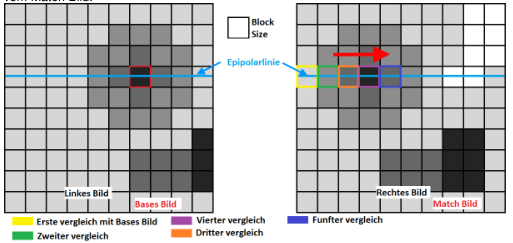
\includegraphics[width=0.8\textwidth]{images/dopracy1.png}  % Adjust the path and width as necessary
    \captionsetup{font=footnotesize}
    \caption[Wyszukiwanie pasujących bloków za pomocą StereoSGBM. Opracowanie własne. ]{Wyszukiwanie pasujących bloków za pomocą StereoSGBM.}
\end{figure}

Im większe dopasowanie między blokiem referencyjnym a blokiem dopasowywanym, tym bardziej prawdopodobne, że odpowiadają one temu samemu punktowi w rzeczywistości.

W tym przykładzie można zauważyć, że blok referencyjny (4,7) ma najwyższy stopień dopasowania z blokiem dopasowywanym (4,4).

W teorii proces powinien przebiegać w ten sposób, jednak w praktyce OpenCV domyślnie analizuje jeszcze 4 inne kierunki, aby uzyskać większą precyzję — stosując tę samą metodę co dla jednego kierunku.

\begin{figure}[H]  % 'h' means "here", it places the figure at the current location in the document
    \centering  % Centers the image
    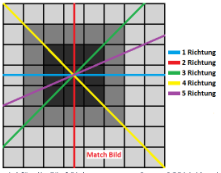
\includegraphics[width=0.5\textwidth]{images/dopracy2.png}  % Adjust the path and width as necessary
    \captionsetup{font=footnotesize}
    \caption[Przykład pięciu kierunków algorytmu StereoSGBM w OpenCV. Opracowanie własne. ]{Przykład pięciu kierunków algorytmu StereoSGBM w OpenCV.}
\end{figure}

Aby znaleźć dysparycję, odejmuje się współrzędne bloku dopasowywanego od współrzędnych bloku referencyjnego, następnie oblicza się wartość bezwzględną wyniku — im większa ta wartość, tym bliżej kamery stereo znajduje się obiekt.

Program używa skalibrowanych obrazów czarno-białych do obliczania mapy dysparycji. Można też pracować z obrazami w formacie BGR, ale wiązałoby się to z większym obciążeniem obliczeniowym dla komputera. Obliczenie mapy odbywa się za pomocą metody obiektu stereo utworzonego wcześniej: cv2.StereoSGBM-create().compute().

Dzięki parametrom ustalonym podczas inicjalizacji otrzymujemy następujący wynik dla mapy dysparycji.

Na tej mapie dysparycji występuje jeszcze sporo szumu. Aby go wyeliminować, stosowany jest filtr morfologiczny. Używany jest filtr typu „Closing” (zamykanie) za pomocą funkcji OpenCV cv2.morphologyEx(cv2.MORPH-CLOSE), aby usunąć małe czarne punkty.

%\begin{figure}[H]  % 'h' means "here", it places the figure at the current location in the document
%    \centering  % Centers the image
%    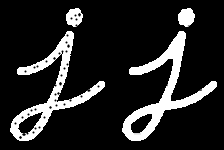
\includegraphics[width=0.5\textwidth]{images/closing.png}  % Adjust the path and width as necessary
%    \captionsetup{font=footnotesize}
%    \caption[Przykład filtra zamykającego. https://docs.opencv.org/3.4/d9/d61/tutorial-py-morphological-ops.html]{Przykład filtra zamykającego.}
%\end{figure}

Poniżej inny przykład tej samej sceny, aby lepiej zobaczyć różnicę.

\subsection{filtr WLS (ważonych najmniejszych kwadratów)}

\begin{lstlisting}[style=mypython]
# WLS FILTER Parameters
wls_filter = cv2.ximgproc.createDisparityWLSFilter(matcher_left=stereo)
wls_filter.setLambda(80000)
wls_filter.setSigmaColor(1.8)
\end{lstlisting}

Wynik nie jest zły, ale wciąż bardzo trudno jest rozpoznać krawędzie obiektów z powodu szumu, dlatego stosowany jest filtr WLS. Na początku należy ustalić parametry filtra podczas inicjalizacji.

Lambda jest zazwyczaj ustawiana na 8000, im wyższa ta wartość, tym bardziej kształty mapy dysparycji będą przypominały kształty obrazu referencyjnego. Ustawiona została wartość na 80000, ponieważ dawało to lepsze wyniki. Sigma opisuje, jak precyzyjny musi być filtr na krawędziach obiektów.

Tworzony jest inny obiekt stereo za pomocą cv2.ximgproc.createRightMatcher(), który opiera się na pierwszym obiekcie. Te dwie instancje są następnie używane w filtrze WLS do generowania mapy dysparycji. Instancja filtra jest tworzona za pomocą funkcji cv2.ximgproc.createDisparityWLSFilter().

Aby zastosować instancję filtra WLS, wywoływana jest następująca metoda: cv2.ximgproc.createRightMatcher().filter(), a wartości naszego filtra są następnie normalizowane za pomocą cv2.normalize().

Zastosowano mapę kolorów Ocean, aby uzyskać lepszą wizualizację, za pomocą cv2.applyColorMap(). Im ciemniejszy kolor, tym dalej znajduje się obiekt od kamery stereo.

W ten sposób otrzymujemy obraz, który dobrze pokazuje krawędzie, ale nie jest już wystarczająco precyzyjny i nie zawiera już dobrych wartości dysparycji (mapa dysparycji jest zakodowana w formacie float32, ale wynik WLS jest zakodowany w uint8).


\subsection{Główna pętla}

\begin{lstlisting}[style=mypython]
while True:

    ret, frame = Cam.read()
    if not ret:
        # Start remap operations in parallel
        break

    height, width, _ = frame.shape
    mid = width // 2

    left_frame = executor.submit(lambda: frame[:, :mid])
    right_frame = executor.submit(lambda: frame[:, mid:])
    LFrame = left_frame.result()
    RFrame = right_frame.result()

    # Start remap operations in parallel
    future_Left_nice = executor.submit(cv2.remap, LFrame, Left_Stereo_Map[0], Left_Stereo_Map[1], interpolation=cv2.INTER_LANCZOS4, borderMode=cv2.BORDER_CONSTANT)
    future_Right_nice = executor.submit(cv2.remap, RFrame, Right_Stereo_Map[0], Right_Stereo_Map[1], interpolation=cv2.INTER_LANCZOS4, borderMode=cv2.BORDER_CONSTANT)
    Left_nice = future_Left_nice.result()
    Right_nice = future_Right_nice.result()

    # Start grayscale conversion in parallel
    future_gray_left = executor.submit(cv2.cvtColor, Left_nice, cv2.COLOR_BGR2GRAY)
    future_gray_right = executor.submit(cv2.cvtColor, Right_nice, cv2.COLOR_BGR2GRAY)
    Gray_left = future_gray_left.result()
    Gray_right = future_gray_right.result()

    # Start disparity computations in parallel
    future_dispL = executor.submit(stereo.compute, Gray_left, Gray_right)
    future_dispR = executor.submit(stereoR.compute, Gray_right, Gray_left)
    DispL = np.int16(future_dispL.result())
    DispR = np.int16(future_dispR.result())

    disp = ((DispL.astype(np.float32) / 16) - min_disp) / num_disp

    filteredImg = wls_filter.filter(DispL, Gray_left, None, DispR)
    filteredImg = cv2.normalize(src=filteredImg, dst=filteredImg, beta=0, 
                                alpha=255, norm_type=cv2.NORM_MINMAX)
    filteredImg = np.uint8(filteredImg)

    filt_Color = cv2.applyColorMap(filteredImg, cv2.COLORMAP_OCEAN)
\end{lstlisting}

Po wygenerowaniu mapy dysparycji należy określić odległość. Zadanie polega na znalezieniu zależności między wartością dysparycji a odległością. Aby to zrobić, eksperymentalnie zmierzyliśmy wartości dysparycji w kilku miejscach, aby na tej podstawie określić regresję.

Aby uzyskać równanie prostej regresji, użyta została biblioteka openpyxl, aby zapisać wartości dysparycji w pliku Excel. Linie w programie, które odpowiadały za zapisanie tych wartości, zostały skomentowane, ale można je odkomentować, jeśli potrzebna jest nowa równość prostej.

\begin{lstlisting}[style=mypython]
_, close_mask = cv2.threshold(filteredImg, 160, 255, cv2.THRESH_BINARY)
close_mask = cv2.morphologyEx(close_mask, cv2.MORPH_CLOSE, kernel)
contours, _ = cv2.findContours(close_mask, cv2.RETR_EXTERNAL, cv2.CHAIN_APPROX_SIMPLE)

for cnt in contours:
    if cv2.contourArea(cnt) > 500:
        x, y, w, h = cv2.boundingRect(cnt)

        roi_disp = disp[y:y + h, x:x + w].astype(np.float32)
        cx, cy = x + w // 2, y + h // 2
        sample_disp = disp[cy - 1:cy + 2, cx - 1:cx + 2].astype(np.float32)
        average_disp = np.mean(sample_disp[sample_disp > 0])

        if average_disp > 0:
            distance = -593.97 * average_disp**3 + 1506.8 
                               * average_disp**2 - 1373.1 
                               * average_disp + 522.06
            distance = np.around(distance * 0.01, decimals=2)

            if distance < 1.0:
                box_color = (0, 0, 255) if distance < 0.5 else (0, 255, 0)
                cv2.rectangle(filt_Color, (x, y), (x + w, y + h), box_color, 2)
                cv2.putText(filt_Color, f"{distance:.2f} m", (x, y - 10),
                            cv2.FONT_HERSHEY_SIMPLEX, 0.5, box_color, 2)
\end{lstlisting}

Pomiar odległości dotyczy tylko odległości od 67 cm do 203 cm, aby uzyskać dobre wyniki. Precyzja pomiaru zależy również od jakości kalibracji. Nasze kamery stereo były w stanie zmierzyć odległość do obiektu z precyzją ± 5 cm.

Zwrócona wartość to średnia dysparycji z macierzy 9x9 pikseli.

\subsection{Wnioski i możliwe ulepszenia}

Możliwe ulepszenia dla programu:

Należy wziąć kształt filtra WLS i projkować go na mapie dysparycji \cite{rao}. Ta projekcja zostanie następnie użyta do pobrania wszystkich wartości dysparycji, które znajdują się w tym kształcie, a wartość, która występuje najczęściej, zostanie ustawiona jako wartość dla całej powierzchni.

Użycie filtra bilateralnego na skalibrowanych obrazach przed wygenerowaniem mapy dysparycji, w ten sposób mogłoby być możliwe, aby nie stosować filtra WLS. Należy to sprawdzić, ale filtr WLS służy głównie do dobrego rozpoznawania krawędzi obiektów, być może istnieje lepsza metoda.

Aby skrócić czas obliczeń przy generowaniu mapy dysparycji, należy zmniejszyć skalibrowane obrazy za pomocą funkcji cv2.resize(cv2.INTER-AbyREA). Należy przy tym pamiętać, że wartości macierzy esencjalnych i fundamentalnych również muszą być proporcjonalnie zmniejszone.

Generowanie mapy głębokości mogłoby również być korzystne.

Wystarczyłoby zapisać wartości macierzy z kalibracji stereo, aby móc je ponownie wykorzystać. Dużo czasu mogłoby to zaoszczędzić w trakcie inicjalizacji.

Uruchomienie programu na GPU pozwoliłoby również uzyskać gładsze obrazy, gdy kamera stereo jest w ruchu.

Aby wartości odległości były zawsze poprawne, należałoby opracować nowy system dla kamer, który zapobiegnie wszelkim swobodnym ruchom kamer. W ten sposób wykorzystywane byłyby tylko wartości macierzy, co przyspieszyłoby proces kalibracji. Używana równość prosta zawsze zwracałaby dokładną odległość do obiektu z większą precyzją i mniejszym nakładem pracy.

\chapter{Zakończenie}

\listoffigures

\begin{thebibliography}{7}
\addcontentsline{toc}{chapter}{Bibliografia}

\bibitem{lambert} John Lambert, Stereo and Disparity, \textit{https://johnwlambert.github.io/stereo/}.
\bibitem{rao} Rajesh Rao, Stereo and 3D Vision, \textit{https://courses.cs.washington.edu/courses/cse455/09wi/Lects/lect16.pdf}.
\bibitem{reilly} Adrian Kaehler, Gary Bradski, Learning OpenCV 3, O'Reilly, 2017-11.
\bibitem{dystorsja} Dystorsja obrazu w fotografii, https://beafoto.pl/dystorsja, 2021-01.
\bibitem{calib} Making A Low-Cost Stereo Camera Using OpenCV, https://learnopencv.com/making-a-low-cost-stereo-camera-using-opencv/, 2021-01-11.

\end{thebibliography}
\end{document}
